%
% `template_basic.tex' - A bare-bones example of using the AIAA class.
%                        For a more advanced usage, see `template_advanced.tex'.
%
% Typical processing for PostScript (PS) output:
%
%  latex template_basic
%  latex template_basic   (repeat as needed to resolve references)
%
%  xdvi template_basic    (onscreen draft display)
%  dvips template_basic   (postscript)
%  gv template_basic.ps   (onscreen display)
%  lpr template_basic.ps  (hardcopy)
%
% With the above, only Encapsulated PostScript (EPS) images can be used.
%
% Typical processing for Portable Document Format (PDF) output:
%
%  pdflatex template_basic
%  pdflatex template_basic      (repeat as needed to resolve references)
%
%  acroread template_basic.pdf  (onscreen display)
%
% If you have EPS figures, you will need to use the epstopdf script
% to convert them to PDF because PDF is a limmited subset of EPS.
% pdflatex accepts a variety of other image formats such as JPG, TIF,
% PNG, and so forth -- check the documentation for your version.
%
% If you do *not* specify suffixes when using the graphicx package's
% \includegraphics command, latex and pdflatex will automatically select
% the appropriate figure format from those available.  This allows you
% to produce PS and PDF output from the same LaTeX source file.
%
% To generate a large format (e.g., 11"x17") PostScript copy for editing
% purposes, use
%
%  dvips -x 1467 -O -0.65in,0.85in -t tabloid template_basic
%
% For further details and support, read the Users Manual, aiaa.pdf.
%
% This software is released under the terms of the LaTeX Project Public
% License.  Copyright (C) 2004 by Bil Kleb, Bill Wood, and Erich Knausenberger.

\documentclass[]{aiaa-tc}% insert '[draft]' option to show overfull boxes

 \title{Bare-Bones \LaTeX\ Template for\\
        AIAA Technical Conference Papers}

 \author{
  First A. Author%
    \thanks{Job Title, Department, Address, and AIAA Member Grade.}
  \ and Second B. Author\thanksibid{1}\\
  {\normalsize\itshape
   Business or Academic Affiliation, City, Province, Zipcode, Country}\\
  \and
  Third C. Author%
   \thanks{Job Title, Department, Address, and AIAA Member Grade.}\\
  {\normalsize\itshape
  Business or Academic Affiliation, City, Province, Zipcode, Country}
 }

 % Data used by 'handcarry' option if invoked
 \AIAApapernumber{YEAR-NUMBER}
 \AIAAconference{Conference Name, Date, and Location}
 \AIAAcopyright{\AIAAcopyrightD{YEAR}}

 % Define commands to assure consistent treatment throughout document
 \newcommand{\eqnref}[1]{(\ref{#1})}
 \newcommand{\class}[1]{\texttt{#1}}
 \newcommand{\package}[1]{\texttt{#1}}
 \newcommand{\file}[1]{\texttt{#1}}
 \newcommand{\BibTeX}{\textsc{Bib}\TeX}

\begin{document}

\maketitle

\begin{abstract}
This is a bare-bones \LaTeX\ template of an AIAA technical conference paper.
It is intended to demonstrate the bare minimum set of \LaTeX\ commands
to produce an AIAA technical conference paper.
To explore more \LaTeX\ capabilities, see the advanced template.
For detailed AIAA layout and style guidelines, please refer to the AIAA
author guide for paper submission, format, and other procedures.
\end{abstract}

\section*{Nomenclature}

\begin{tabbing}
  XXX \= \kill% this line sets tab stop
  $J$ \> Jacobian Matrix \\
  $f$ \> Residual value vector \\
  $x$ \> Variable value vector \\
  $F$ \> Force, N \\
  $m$ \> Mass, kg \\
  $\Delta x$ \> Variable displacement vector \\
  $\alpha$ \> Acceleration, m/s\textsuperscript{2} \\[5pt]
  \textit{Subscript}\\
  $i$ \> Variable number \\
 \end{tabbing}

\section{Introduction}

This would be a good place to insert some text that make sense relative
to the paper being written.
Of course, for example purposes, the text is quite meaningless.


\section{Feasible Path Generation}


Real-time path generation that explicitly accounts for dynamic
constraints is a critical requirement for the autonomous vehicles
of today. In this section, we describe a path generation algorithm
that is suitable for real-time computation of feasible
trajectories for multiple UAVs that are de-conflicted in space and
that can be followed by resorting to the path following algorithm
described later in the paper. The key ideas involved can be best
explained with the help of an example. Consider a fleet of $n$
UAVs that are tasked to start from different locations and arrive
at the same final target simultaneously. The exact time of arrival
is not specified, but it may be restricted to lie within certain
bounds.

Suppose the objective is to execute this multi-vehicle mission
while avoiding inter-vehicle collisions, meeting dynamical
constraints (e.g. bounds on maximum accelerations), and minimizing
a weighted combination of vehicle energy expenditures. At first
inspection, a possible solution to this problem would be to solve
a constrained optimization problem that would yield (if at all
possible) feasible trajectories $p_{c_i}(t), t \in [0, t_f];
i=1,2,...,n$ for the vehicles, where $t_f$ denotes the final time.
Trajectory tracking systems on-board the UAVs would then ensure
precise tracking of the trajectories generated, thus meeting the
mission objectives.

This seemingly straightforward solution suffers from a major
drawback: it does not allow for any ``deviations from the plan''.
Absolute timing becomes crucial because the strategy described
does not lend itself to on-line modification in the event that one
or more of the vehicles cannot execute trajectory tracking
accurately (e.g. due to adverse winds or lack of sufficient
propulsion power). For this reason, it is far more practical to
adopt a different solution where absolute time is not crucial and
enough room is given to each vehicle to adjust its motion along
the path in response to the motions of the other vehicles. The
goal is that of reaching a terminal formation pattern that will
ensure simultaneous arrival times. Dispensing with absolute time
is key to the solution proposed. In this set-up, the optimization
process should be viewed as a method to produce paths
$p_{c_i}(\tau_i)$ without explicit time constraints, but with
timing laws for $\tau_i(t)$ that effectively dictate how the
nominal speed of each vehicle should evolve along the path. Using
this set-up, spatial and temporal constraints are essentially
decoupled and captured in the descriptions of $p_{c_i}(\tau_i)$
and $\eta_i(\tau_i)=d\tau_i/dt$, respectively, as will be seen
later. Furthermore, adopting polynomial approximations for
$p_{c_i}(\tau_i)$ and $\eta_i(\tau_i)=d\tau_i/dt$ keeps the number
of optimization parameters reduced and makes real-time
computational requirements easy to achieve. Intuitively, by making
the path of a generic vehicle a polynomial function of  $\tau \in
\ [0, \tau_f ]$, the shape of the path in space can be changed by
increasing or decreasing $\tau$ - a single optimization parameter.
This, coupled with a polynomial approximation for
$\eta(\tau)=d\tau/dt$, makes it easy to shape the speed and
acceleration profile of the vehicle along the path so as to meet
desired dynamical constraints. The paths thus generated are the
``templates'' used for path following, as explained in Section
II.B later in the paper.

%In particular, In addition, the vehicle's velocity and acceleration
%can be easily computed along this path. If the path length is too
%short, vehicle's velocity and acceleration will exceed the
%pre-specified bounds thus making the trajectories infeasible -
%impossible for vehicle to track given its dynamic constraints. This
%simple idea allows for computing feasible trajectories in real-time
%using a small number of optimization parameters.


The above circle of ideas was first explored in Refs.
\cite{Neljubov, Taranenko, Taranenko-Momdgi, Yakimenko} for a
single aircraft. This paper extends these results to the case of
multiple UAVs following earlier work by the authors reported in
Ref. \cite{isaac_acc_06}. As will be seen, the approach to path
generation exploits a separation between spatial and temporal
specifications. Let $p_c(\tau) = [x(\tau), y(\tau),
z(\tau)]^{\top}$ denote a desired path to be followed by a single
UAV, parameterized by $\tau \in [0, \tau_f]$. For computational
efficiency, assume each coordinate $x (\tau), y(\tau), z(\tau)$ is
represented by an algebraic polynomial of degree $N$ of the form
\begin{eqnarray} \label{algpolynomials} x_{i}(\tau) &=& \sum_{k =
0}^{N} a_{ik} \tau^k, \qquad i = 1,2,3, \end{eqnarray} where we
set $x_{1} = x, x_{2} = y, x_{3} = z$ for notational convenience.
The degree $N$ of polynomials $x_{i}(\tau)$ is determined by the
number of boundary conditions that must be satisfied. Notice that
these conditions (that involve spatial derivatives) are computed
with respect to the parameter $\tau$. There is an obvious need to
relate them to actual temporal derivatives, but this issue will
only be addressed later. For the time being, let $d_0$ and $d_f$
be the highest-order of the spatial derivatives of $x_{i}(\tau)$
that must meet specified boundary constraints at the initial and
final points of the path, respectively. Then, the minimum degree
$N^*$ of each polynomial in (\ref{algpolynomials}) is $N^{*} = d_0
+ d_f + 1$. For example, if the desired path includes constraints
on initial and final positions, velocities, and accelerations
(second-order derivatives), then the degree of each polynomial is
$N^{*} = 2 + 2 + 1 = 5$. Explicit formulae for computing boundary
conditions $p'_c(0), p''_c(0)$ and $p'_c(\tau_f), p''_c(\tau_f)$
are given later in this section.  Additional degrees of freedom
may be included by making $N > N^*$. As an illustrative example,
Table 1 shows how to compute the polynomial coefficients in
(\ref{algpolynomials}) for polynomial trajectories of $5^{{\rm
th}}$ and $6^{{\rm th}}$ degree. For $6^{{\rm th}}$ degree
polynomial trajectories,  an additional constraint on the
fictitious initial jerk (third-order derivatives) is included,
which increases the order of the resulting polynomial and affords
extra (design) parameters $ x'''_{i}(0); i = 1,2,3$.  Fig.
\ref{trajsim1} shows examples of admissible $5^{{\rm th}}$ and
$6^{{\rm th}}$ order polynomial paths when only $\tau_f$ or
$\tau_f$ and $x'''_{i}(0); i = 1,2,3$, viewed as optimization
parameters, vary. Fig. \ref{trajsim1} (right) shows how an
increase in the number of optimization parameters leads to a
larger class of admissible paths (in this particular case,
parameters corresponding to initial jerk are added as free
variables).



%The fact that the virtual arc $\tau$ was selected as a parameter in
%(\ref{algpolynomials}) allows for additional flexibility. If one
%chooses $\tau = t$, then defining spatial profiles implies defining
%speed profiles along a given path as well. This is due to the fact
%that vehicle speed along the path is related to the time derivatives
%of the trajectory coordinates as
%\begin{eqnarray} \label{velocity} v(t) &=& \sqrt{ \dot{x}_{1}^2(t)
%+ \dot{x}^2_{2}(t) + \dot{x}^2_{3}(t)}. \end{eqnarray} Figure
%\ref{speedsims1} shows the speed profiles corresponding to the
%trajectories in Figure \ref{trajsim1} for the case of $\tau = t$.
%This figure also demonstrates that increasing the number of
%optimization parameters allows one to obtain speed profiles that do
%not exceed predefined constraints.





It is now important to clarify how temporal constraints may be
included in the feasible path computation process. A trivial
solution would be to make $\tau=t$. In this case, solving the
polynomial fitting problem that is at the root of Fig.
\ref{trajsim1} yields the speed profiles of Fig. \ref{speedsims1}.
Little control exists over the resulting speeds even with fifth
and sixth order polynomials, because once $x_1(t), x_2(t), x_3(t)$
have been computed to satisfy the boundary constraints imposed,
speed $v$ is inevitably given by
\begin{eqnarray}
\label{velocity} v(t) &=& \sqrt{ \dot{x}_{1}^2(t) +
\dot{x}^2_{2}(t) + \dot{x}^2_{3}(t)}.
\end{eqnarray}

We therefore turn our attention to a different procedure that will
afford us the possibility of meeting strict boundary conditions
and constraints without increasing the complexity of the path
generation process. To this effect, let $v_{{\rm min}}, v_{{\rm
max}}$ and $a_{{\rm max}}$ denote predefined bounds on the
vehicle's speed and acceleration, respectively. Let $\eta(\tau) =
d\tau/dt$, yet to be determined, dictate how parameter $\tau$
evolves in time. A path $p_c(\tau)$ (with an underlying assignment
$\eta(\tau)$) is said to constitute a \textit{feasible} path if
the resulting trajectory can be tracked by an UAV without
exceeding prespecified bounds on its velocity and total
acceleration along that trajectory. With an obvious use of
notation, we will later refer to a spatial path only, without the
associated $\eta(\tau)$, as a feasible path.

>From (\ref{velocity}), and for a given choice of $\eta(\tau)$, the
temporal speed $v_p(\tau(t))$ and acceleration $a_p(\tau(t))$ of
the vehicle along the path (abbv. $v_p(\tau)$ and $a_p(\tau)$,
respectively) are given by

\begin{eqnarray} \nonumber
v_p(\tau) \hspace{ -0.2 cm} &=& \hspace{ -0.2 cm} \eta(\tau)
\sqrt{x'^2_{1}(\tau) + x'^2_{2}(\tau) + x'^2_{3}(\tau)} ~ = ~
\eta(\tau) ||p'_c(\tau)||, \\
\label{velacc} a_p(\tau) \hspace{ -0.2 cm} &=& \hspace{ -0.2 cm}
=||\ddot{p}_c(t) || = ||p''_c(\tau) \eta^2(\tau) + p'_c(\tau) \eta'(\tau)  \eta(\tau)||.
\end{eqnarray}


\begin{tabular}{cc}
\multicolumn{2}{l}{Table 1.  Examples of computation of the
coefficients
of $5^{{\rm th}}$ and $6^{{\rm th}}$ order polynomial paths.} \\
\hline \multicolumn{2}{c}{$5^{{\rm th}}$ order} \\ \hline \\
Boundary conditions & $x_{i}(0), x'_{i}(0), x''_{i}(0), x_{i}(\tau_f), x'_{i}(\tau_f), x''_{i}(\tau_f)$ \\
$d_0/d_f$                 & 2/2 \\
$N^*/N$                   & 5/5 \\ \\
\begin{tabular}{ c }
Linear algebraic matrix \\
equation to solve for the \\
coefficients $a_{ik}$ \end{tabular}
                           & $\left[ \begin{array}{cccccc}
                            1 & 0 & 0 & 0 & 0 & 0 \\
                            0 & 1 & 0 & 0 & 0 & 0 \\
                            0 & 0 & 2 & 0 & 0 & 0 \\
                            1 & \tau_f & \tau^2_f & \tau^3_f & \tau^4_f & \tau^5_f \\
                            0 & 1 & 2 \tau_f & 3 \tau^2_f & 4 \tau^3_f & 5 \tau^4_f \\
                            0 & 0 & 2 & 6 \tau_f & 12 \tau^2_f & 20 \tau^3_f
                            \end{array} \right] \left[
                            \begin{array}{cccccc}
                            a_{i0} \\ a_{i1} \\ a_{i2} \\ a_{i3}
                            \\ a_{i4} \\ a_{i5} \end{array}
                            \right] = \left[
                            \begin{array}{cccccc}
                            x_{i}(0) \\ x'_{i}(0) \\ x''_{i}(0) \\
                            x_{i}(\tau_f) \\ x'_{i}(\tau_f) \\
                            x''_{i}(\tau_f) \end{array} \right]$ \\
                            \\
                            \hline
\multicolumn{2}{c}{ $6^{{\rm th}}$ order} \\ \hline \\


Boundary conditions & $x_{i}(0), x'_{i}(0), x''_{i}(0), x'''_{i}(0), x_{i}(\tau_f), x'_{i}(\tau_f), x''_{i}(\tau_f)$ \\
$d_0/d_f$                 & 3/2 \\
$N^*/N$                   & 5/6 \\ \\
\begin{tabular}{ c }
Linear algebraic matrix \\
equation to solve for the \\
coefficients $a_{ik}$ \end{tabular}
                          & $\left[ \begin{array}{ccccccc}
                            1 & 0 & 0 & 0 & 0 & 0 & 0 \\
                            0 & 1 & 0 & 0 & 0 & 0 & 0 \\
                            0 & 0 & 2 & 0 & 0 & 0 & 0 \\
                            0 & 0 & 0 & 6 & 0 & 0 & 0 \\
                            1 & \tau_f & \tau^2_f & \tau^3_f & \tau^4_f & \tau^5_f & \tau^6_f \\
                            0 & 1 & 2 \tau_f & 3 \tau^2_f & 4 \tau^3_f & 5 \tau^4_f & 6 \tau^5_f \\
                            0 & 0 & 2 & 6 \tau_f & 12 \tau^2_f & 20
                            \tau^3_f & 30 \tau^4_f
                            \end{array} \right] \left[
                            \begin{array}{ccccccc}
                            a_{i0} \\ a_{i1} \\ a_{i2} \\ a_{i3}
                            \\ a_{i4} \\ a_{i5} \\ a_{i6} \end{array}
                            \right] = \left[
                            \begin{array}{ccccccc}
                            x_{i}(0) \\ x'_{i}(0) \\ x''_{i}(0) \\
                            x'''_{i}(0) \\ x_{i}(\tau_f) \\ x'_{i}(\tau_f) \\
                            x''_{i}(\tau_f) \end{array} \right]$







%
%  \caption{Examples of computation of the coefficients of polynomial trajectories.}\label{polynomialtable}
%  \centering
 \end{tabular} \\ \\







\begin{figure}\begin{center}
  % Requires \usepackage{graphicx}
  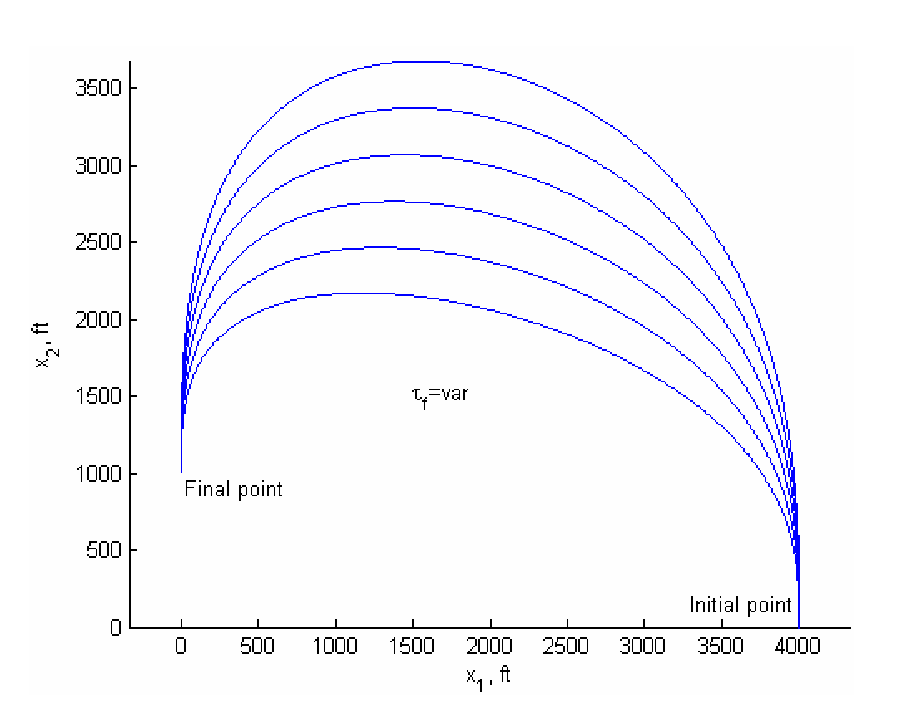
\includegraphics[width=2.5 in]{figures/poly1.eps}   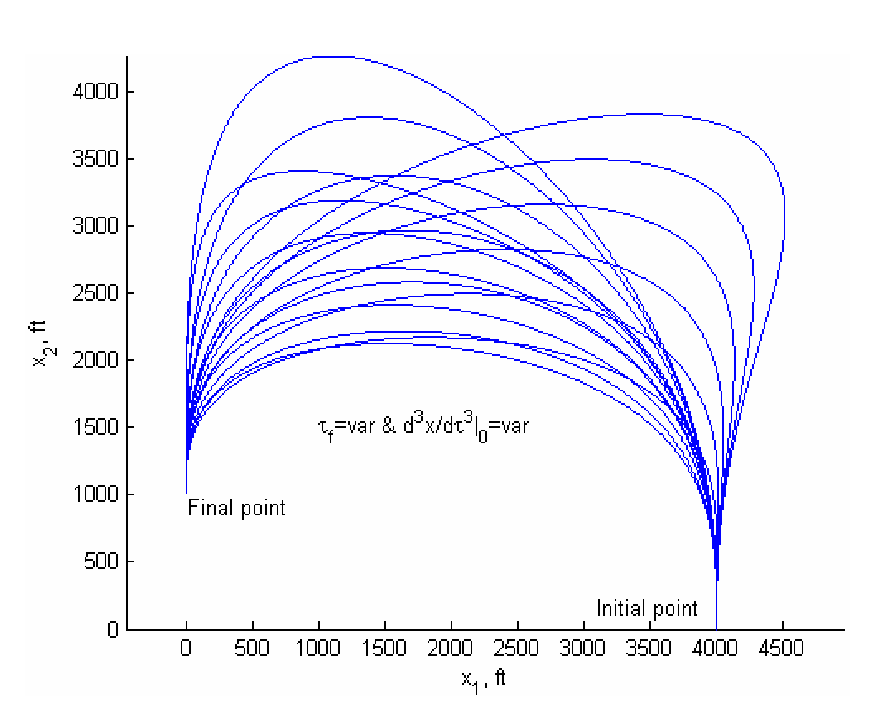
\includegraphics[width=2.5 in]{figures/poly2.eps}\\
  \caption{Admissible trajectories for $5^{{\rm th}}$ and $6^{{\rm th}}$ order
  polynomials.}\label{trajsim1}\end{center}
\end{figure}

\begin{figure}\begin{center}
  % Requires \usepackage{graphicx}
  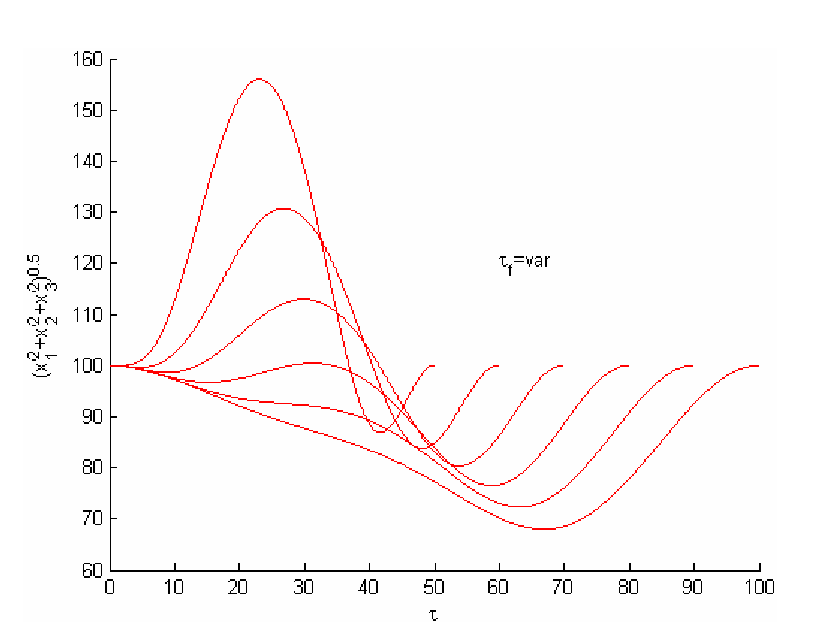
\includegraphics[width=2.6 in]{figures/traj1.eps}   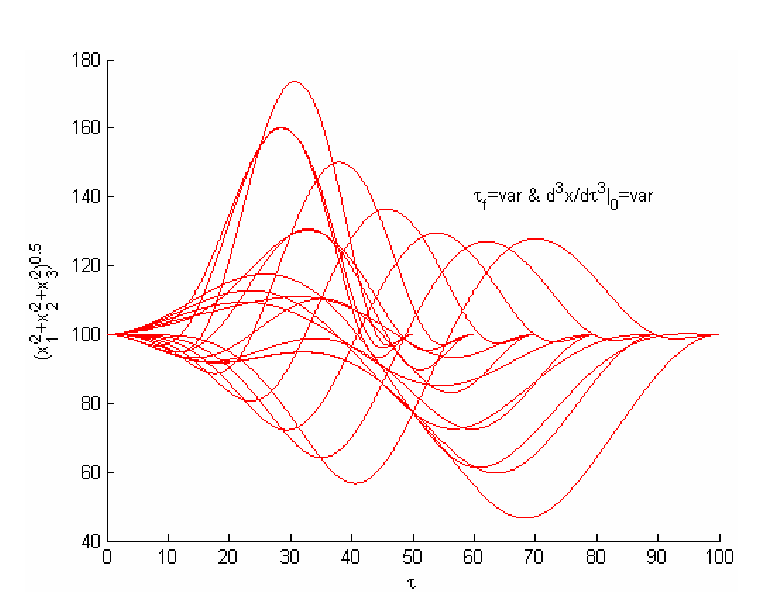
\includegraphics[width=2.6 in]{figures/traj2.eps}\\
  \caption{Speed profile corresponding to the paths shown in Figure \ref{trajsim1} when $\tau =
  t$. Left: varying $\tau_f$. Right: varying $\tau_f$ and the initial
jerk.}\label{speedsims1}.
  \end{center}
\end{figure}

% IK changes

In this paper we are interested in small UAVs that operate essentially at constant speeds.
Clearly, in this case speed constraints can be easily satisfied for any constant $ v_p \in [v_{{\rm min}}, v_{{\rm max}} ]$. This in turn defines

\begin{eqnarray}
\eta(\tau) &=&  \frac{v_p}{||p'_c(\tau)||} \label{defeta}\\
%\eta'(\tau)&=& -v_p \frac{(p'_c(\tau))^T p''_c(\tau)}{|| p'_c(\tau)||^3}.
\dot p_c(t) &=& v_p \frac{p'_c(\tau)}{|| p'_c(\tau)||} \label{ptau}
\end{eqnarray}

\noindent Now using (\ref{velacc}, \ref{defeta}) we obtain

\begin{eqnarray}
\ddot{p}_c(t)&=&\frac{v_p^2}{||p'_c(\tau)||^2} (I - \frac{p'_c(\tau)
(p'_c(\tau))^T}{||p'_c(\tau)||^2}) p''(\tau). \label{pptau}
\end{eqnarray}

\noindent Therefore, we can choose
\begin{eqnarray}
p'_c(0) &=& \frac{\dot p_c(0)}{||\dot p_c(0)||} \label{ptau0} \\
p'_c(\tau_f) &=& \frac{\dot p_c(t_f)}{||\dot p_c(t_f)||}.
\label{ptauf}
\end{eqnarray}
\noindent to satisfy boundary conditions on $\dot p_c(t)$. Similarly, setting
\begin{eqnarray*}
p''_c(0) &=& \ddot p_c(0) \label{pptau0} \\
p''_c(\tau_f) &=& \ddot p_c(t_f)  \label{pptauf}, \\
\end{eqnarray*}
satisfies equation (\ref{pptau}) at the boundaries.

On the other hand, the total acceleration $a_p$
of a vehicle flying along the path $p_c(\tau)$ at a constant speed is the product of the curvature of
the path with its velocity along the path squared. The curvature of the path $p_c(\tau)$ is given by
\[
\kappa(\tau) = \frac{1}{||p'(\tau)||}
||\frac{d}{d \tau} \frac {p'_c(\tau)}{||p'_c(\tau)||}||.
\]
\noindent Thus, using simple algebra it can be shown that
\begin{eqnarray*}
a_p(\tau) &=& v^2_p \kappa(\tau) \\
    &=&\frac{v_p^2}{||p'_c(\tau)||^2}
||(I - \frac{p'_c(\tau)(p'_c(\tau))^T}{||p'_c(\tau)||^2}) p''(\tau)||,
\end{eqnarray*}
\noindent which as expected is the norm of $\ddot p_c(t)$ (see equation (\ref{pptau}).
Therefore, for the case of constant
velocities $v_p$ a feasible path must satisfy the following set
of constraints

\begin{eqnarray} \label{cond1a}
v_{\rm min} \le v_p ~ \le v_{\rm max}, ~~~~ a_p(\tau) \le a_{\rm max},
~ \forall \tau \in [0,\tau_f].
\end{eqnarray}

\noindent for a pre-specified acceleration bound $a_{\rm max}$.

In this paper, we use the freedom afforded by a simple definition of a feasible path above to address the problem of
time-coordinated control of multiple UAVs whereby all UAV's must arrive at their
respective final destinations at the same time.  The approach proposed here seeks to find a set of feasible paths that makes the coordinated arrival time problem easily solvable by a team of UAVs flying at constant speeds along these paths while coordinating their motion using the underlying communication network. In particular, these paths should be designed in such a way as to guarantee the simultaneous arrival by all UAVs at their respective destinations. Next, we make these ideas more precise.

Let $l_{fi}$ denote the total path length of the $ith$ path and
$v_{p_i}$ denote its velocity along this path. Then
$$
l_{fi}=\int^{\tau_{fi}}_0 ||p'_{c_i}(\tau_i)|| ~ d \tau_i.
$$
It follows immediately that the time of flight $t_{fi}$ of UAV $i$ is given by
\begin{eqnarray} \nonumber t_{fi_{{\rm min}}} &=&
\int^{\tau_{fi}}_0 \frac{||p'_{c_1}(\tau_i)||} {v_{{\rm p}_{i}}}~ d \tau_i .
\end{eqnarray}
Define a cost function $J = (\max_i t_{fi} - \min_i t_{fi})^2$. Then, making $J$ arbitrarily small over the set of feasible paths, feasible velocities and accelerations  will
result in the desired solution to the simultaneous arrival problem
discussed above. Therefore, we propose to solve the following
path generation problem

\begin{eqnarray}
F1: \left\{
\begin{array}{llll}
\displaystyle{\min_{\tau_{fi},v_{p_i}, \; i =1,\ldots,n} \{ J  \} } \\ \\
~~ ~ subject ~
to \\ \\
~ boundary ~ conditions ~ and ~(\ref{cond1a}) ~ for~ any ~ i
\in [1,n] \\ \\
\displaystyle{\min_{j,k = 1, \ldots, n, j \ne k} ||
p_{c_j}(\tau_j) - p_{c_k}(\tau_k)||^2 \ge E^2 ~ for ~ any ~
\tau_j, \tau_k \in [0,
\tau_{fj}] \times [0, \tau_{fk}]},
\end{array} \right.
\end{eqnarray}

Solution to the optimization problem $F1$ includes a set of $n$ optimal paths and constant speed profiles that together minimize $J$ subject to an additional constraint that these paths must be spatially separated by at least $E$ meters:
$\displaystyle{\min_{j,k = 1, \ldots, n, j \ne k} || p_{c_j}(\tau_j)
- p_{c_k}(\tau_k)||^2 \ge E^2 ~ for ~ any ~ \tau_j, \tau_k \in [0,
\tau_{fj}] \times [0, \tau_{fk}]}$
Clearly, this constraint guarantees collision avoidance.


The optimization problem $ F1$ can be effectively solved in
real-time by adding a penalty function $G$ as discussed in Ref.
\cite{Yakimenko} and by using any zero-order optimization
technique. As an example, Fig.~\ref{ex1} illustrates the
flexibility afforded by the reference polynomials to compute a
coordinated target reconnaissance mission by three UAVs. In this
case, the vector of optimization parameters is $\Xi = [\tau_{f1}
~~ \tau_{f2} ~~ \tau_{f3} ~~ v_{p_1} ~~ v_{p_2}~~ v_{p_3}]$. The
final value of the cost function $J = 1.6968e-006$ corresponds to
$|\max_i t_{fi} - \min_i t_{fi}| \le ~~ 0.0013 ~~ sec$. The value
of the optimization parameter vector $\Xi_{final} = [4010.0 ~~
4999.7 ~~ 7487.6 ~~ 15.1380 ~~ 21.2238 ~~ 29.8054]$ resulted in
spatially deconflicted paths where the minimum distance between
any two paths did not fall below $350 ~ m$ (the minimum required
distance was $100 ~ m$). The optimal speed profiles $[15.1380~m/s
~~ 21.2238~m/s ~~ 29.8054~m/s]$ are well within predefined limits
of $v_{{\rm min}}, v_{{\rm max}}$ were $15 m/sec$ and $30 m/sec$,
respectively.
%The selected speed limits were
%well inside the physical capabilities of the UAVs used in the flight
%tests.
%This was done to ensure that each path can be tracked in
%the presence of winds.
The maximum acceleration corresponding to
each path did not exceed $0.89 m/sec^2$, well below the limit of
$0.5 g$.  Finally, the resulting total path lengths for each path were
$[ \l_{f1} ~~ \l_{f2} ~~ \l_{f3} ] = [4535.4 ~~ 6358.7  ~~ 8929.7]$.




%\begin{figure}
%  % Requires \usepackage{graphicx}
%  \begin{center}
%  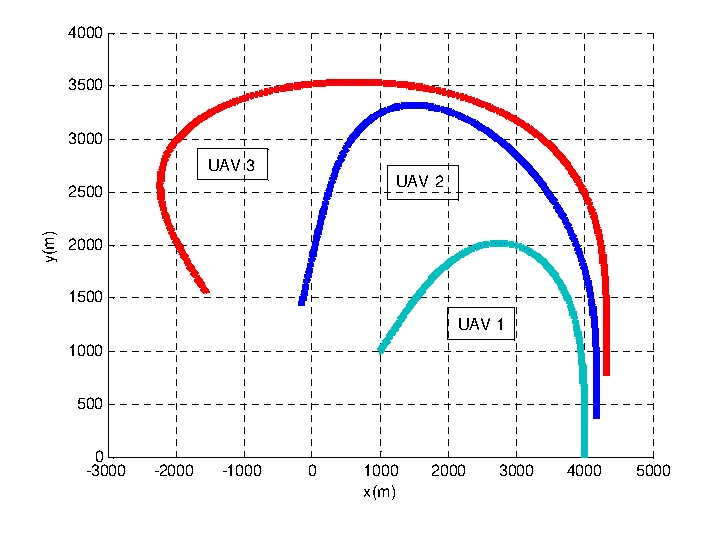
\includegraphics[width=3in]{traj3.eps}
%  \includegraphics[width=3.2in]{traj4.eps}
%  \caption{Example of spatially deconflicted trajectories.  Top view, moving from right to left (left), 3D view, moving from left to right (right).}\label{ex1}
%\end{center} \end{figure}
%
%
%\begin{figure}
%  % Requires \usepackage{graphicx}
%  \begin{center}
%  \includegraphics[width=3.1in]{traj6.eps}\\
%  \caption{Intersection of time intervals $T_i$ for each UAV.}\label{ex3}
%\end{center} \end{figure}



\begin{thebibliography}{9}% maximum number of references (for label width)
 \bibitem{rebek:82bk}
 Rebek, A., {\it Fickle Rocks}, Fink Publishing, Chesapeake, 1982.
\end{thebibliography}

\end{document}

% $Id: template_basic.tex,v 1.5 2004/05/23 12:49:44 kleb Exp $
